\documentclass[12pt]{article}
\usepackage[margin=1in]{geometry}
\usepackage{graphicx}
\usepackage{amsmath,amssymb}
\pagestyle{empty}
\begin{document}

\begin{center}
\textbf{\large Online Resource 1}
\end{center}
\vspace{0.5em}

\begin{center}
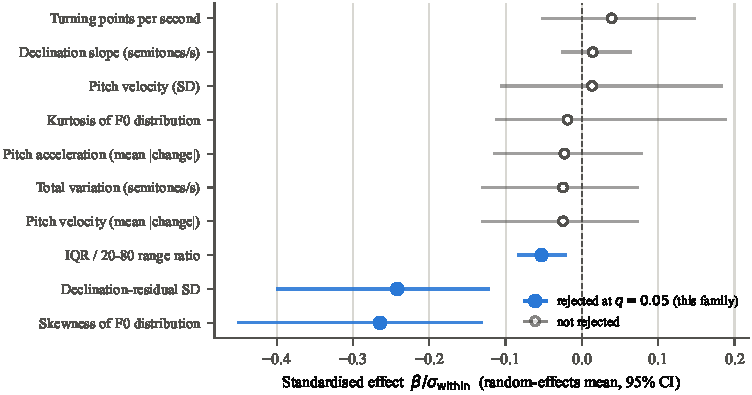
\includegraphics[width=0.85\textwidth]{fig_tier12.pdf}
\end{center}

\vspace{1em}
\noindent\textbf{Caption.} Within-debate standardized effect (random-effects
mean, $95\%$ confidence interval) for the ten higher-order and dynamic
pitch-contour measures reported in Table~6 of the main text
(``Primary Result''). Filled markers survive Benjamini-Hochberg correction
within this family of measures. This figure presents, in visual form, the
same effect sizes tabulated in Table~6 of the main text.

\end{document}
